\section{Solving the Diffusion Equation for Iron Poker}
\label{sec:diffusion_equation}

In the final section of the exercise, the heat diffusion equation is solved for a metal rod. The heat diffusion equation is given by:
\begin{equation}
    \alpha \nabla^2 \phi = \frac{\partial \phi}{\partial t},
\end{equation}
where $\alpha = \frac{k}{\rho c_p}$ (with $k$ the the thermal conductivity, $\rho$ the density and $c_p$ the specific heat capacity) is the thermal diffusivity and $\phi$ is the temperature. Two boundary conditions are solved for: firstly, one end in a hot furnace of \SI{1000}{\celsius} only, and the other with one end in a hot furnace of \SI{1000}{\celsius} and the other in cold ice at \SI{0}{\celsius}. Heat loss through the edges of the rod are ignored throughout.

\subsection{One end held in furnace at \SI{1000}{\celsius}}
\label{subsec:hot}

Firstly, one end of the rod is held in a furnace of temperature \SI{1000}{\celsius}, and no heat is lost through the end of the poker. The result of letting time advance is thus to let heat gradually dissipate up through the rod to the other end of the rod. Because no heat is lost, heat continues to build up indefinitely until the entire rod is at \SI{1000}{\celsius}. Whilst the rod will never in a finite time reach this equithermal point, the entire rod is at the same temperature to an absolute error tolerance of $\epsilon = 10^{-4}$\si{\kelvin} after 261,322 iterations with step size \SI{0.1}{\second}, i.e. after \SI{26,132}{\second}. Figures \ref{fig:hot_diffusion} show the one-dimensional temperature distribution along the rod as time advances.

\begin{figure}
    \centering
    \subfloat[$t=$\SI{10}{\second}]{
        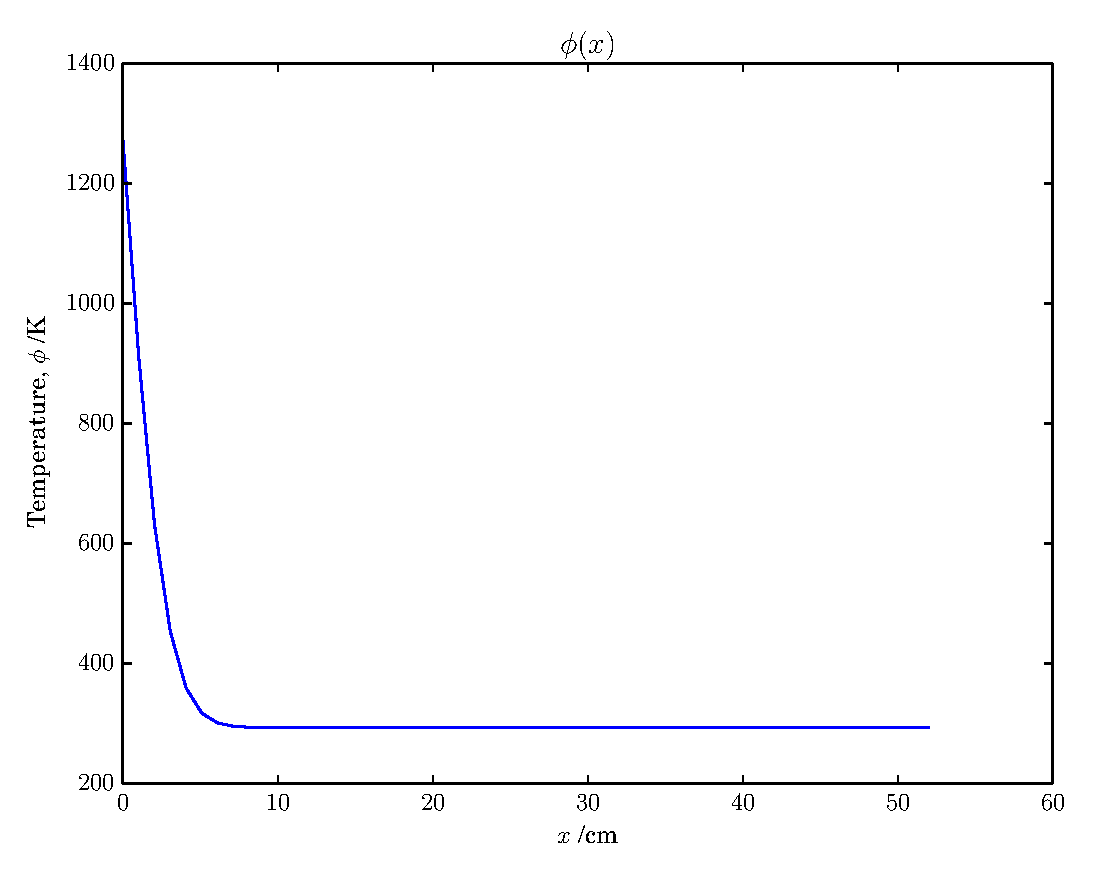
\includegraphics[width=0.5\linewidth]{graphs/diffusion/hot/t_10_rod_normal}
    }
    \subfloat[$t=$\SI{100}{\second}]{
        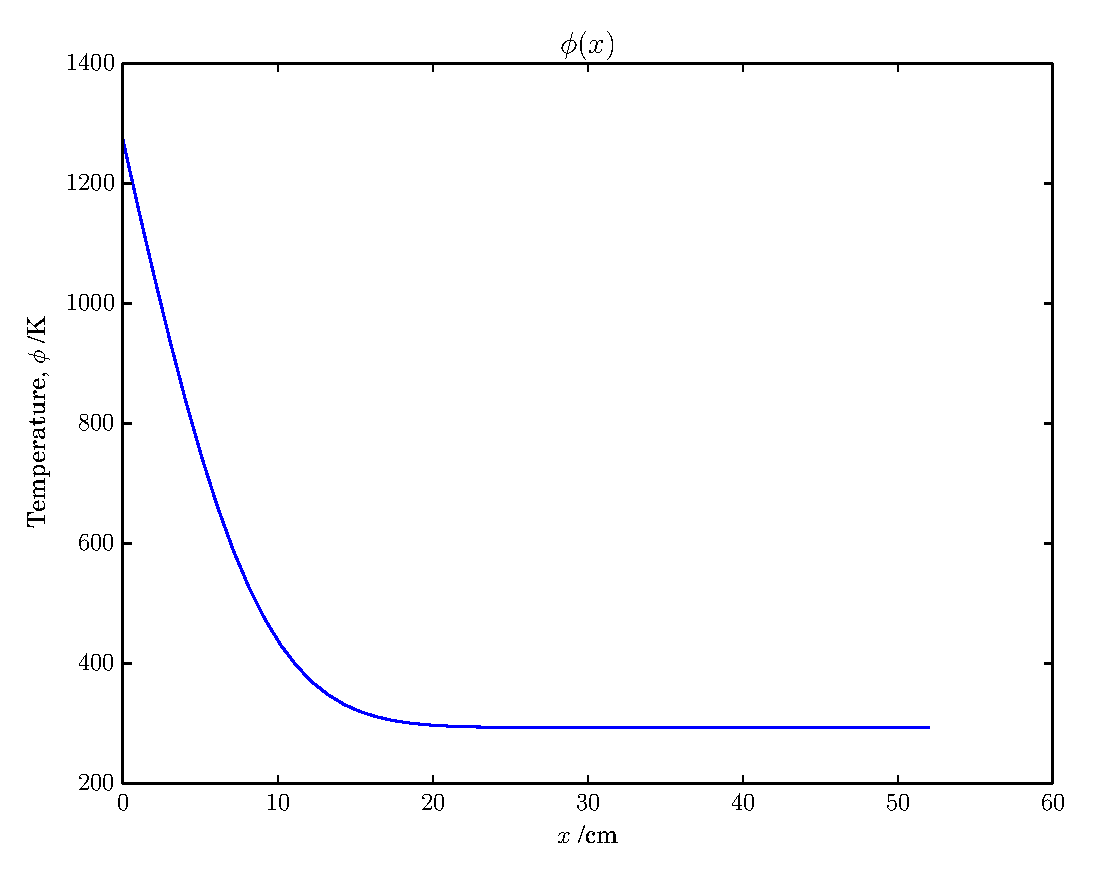
\includegraphics[width=0.5\linewidth]{graphs/diffusion/hot/t_100_rod_normal}
    }
    \caption{Temperature distribution along rod with one end in furnace at \SI{10}{\second} and \SI{100}{\second}.}
\end{figure}

\begin{figure}
    \ContinuedFloat
    \centering
    \subfloat[$t=$\SI{1000}{\second}]{
        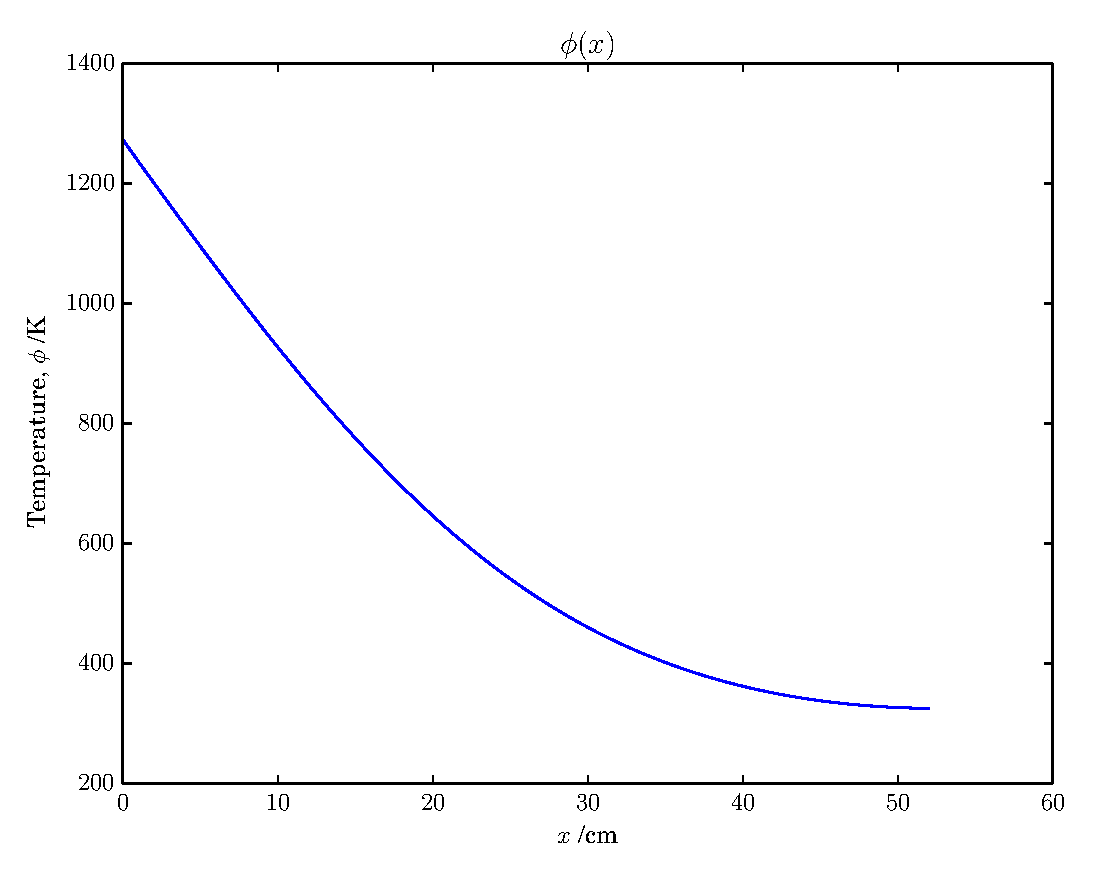
\includegraphics[width=0.5\linewidth]{graphs/diffusion/hot/t_1000_rod_normal}
    }
    \subfloat[$t=$\SI{10000}{\second}]{
        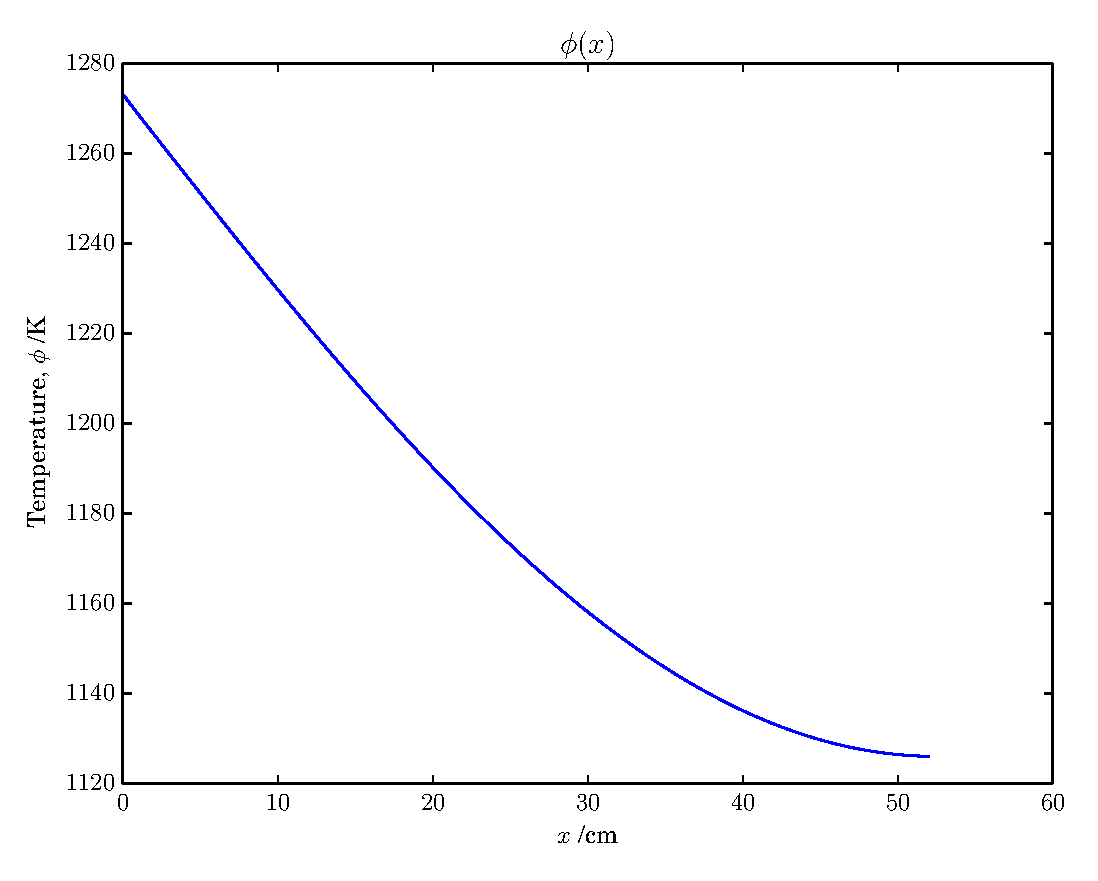
\includegraphics[width=0.5\linewidth]{graphs/diffusion/hot/t_10000_rod_normal}
    }
    \caption{Temperature distribution along rod with one end in furnace at \SI{1000}{\second} and \SI{10000}{\second}.}
    \label{fig:hot_diffusion}
\end{figure}

\subsection{Other end held in ice at \SI{0}{\celsius}}
\label{subsec:cold}

Once the other end of the rod is submerged in ice at \SI{0}{\celsius}, the time evolution of the temperature distribution of the rod drastically changes. Where before no true equilibrium can be found in finite time (ignoring floating point errors), the existence of the boundary condition of the ice means that after 7206.9 seconds, the system converges to an equilibrium state, where the temperature distribution function linearly falls off from \SI{1000}{\celsius} at one end to \SI{0}{\celsius} at the other end, as shown in Figure \ref{subfig:cold_t_10000}. The time advancement shown in Figure \ref{fig:cold_diffusion} is similar to that of \ref{fig:hot_diffusion}, however the fall-off is skewed at the right hand side due to the presence of the cold ice on the right end of the rod.

\begin{figure}
    \centering
    \subfloat[$t=$\SI{10}{\second}]{
        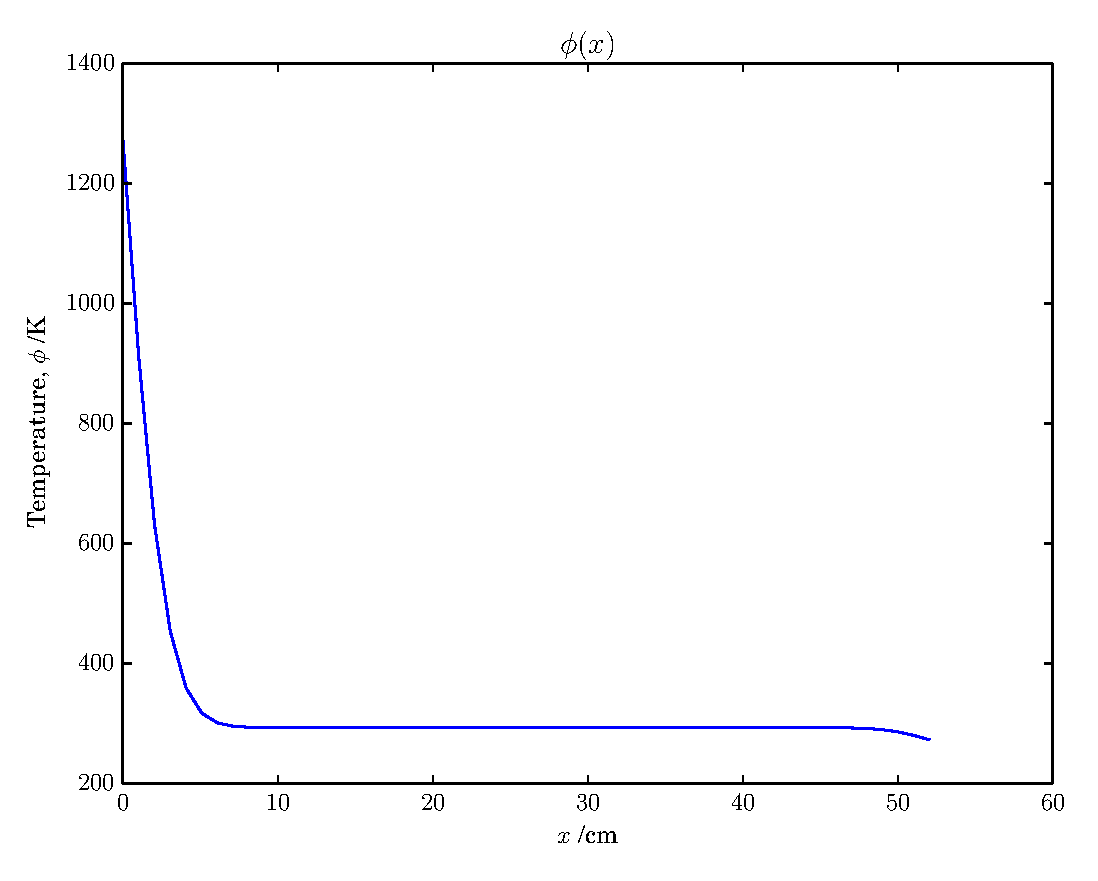
\includegraphics[width=0.5\linewidth]{graphs/diffusion/cold/t_10_rod_normal}
        \label{subfig:cold_t_10}
    }
    \subfloat[$t=$\SI{100}{\second}]{
        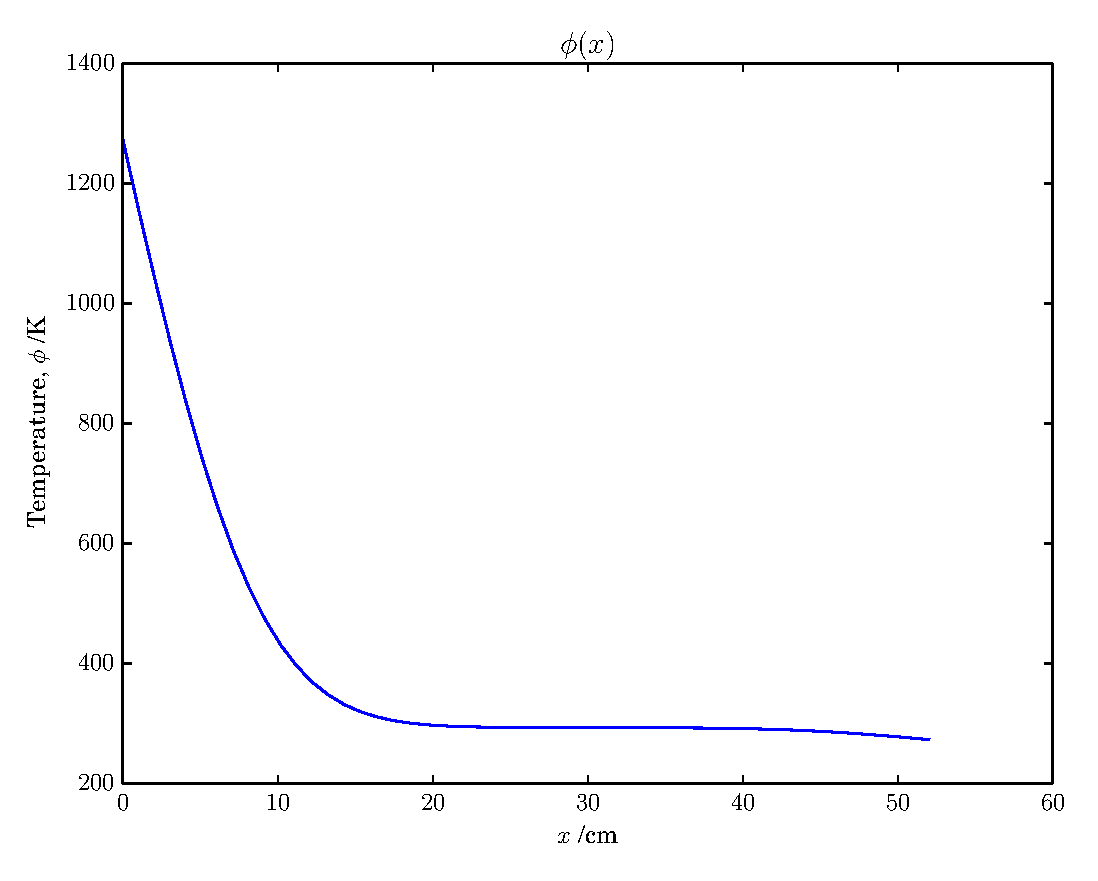
\includegraphics[width=0.5\linewidth]{graphs/diffusion/cold/t_100_rod_normal}
        \label{subfig:cold_t_100}
    }
    \caption{Temperature distribution along rod with one end in furnace and other in ice at \SI{10}{\second} and \SI{100}{\second}.}
\end{figure}

\begin{figure}
    \ContinuedFloat
    \centering
    \subfloat[$t=$\SI{1000}{\second}]{
        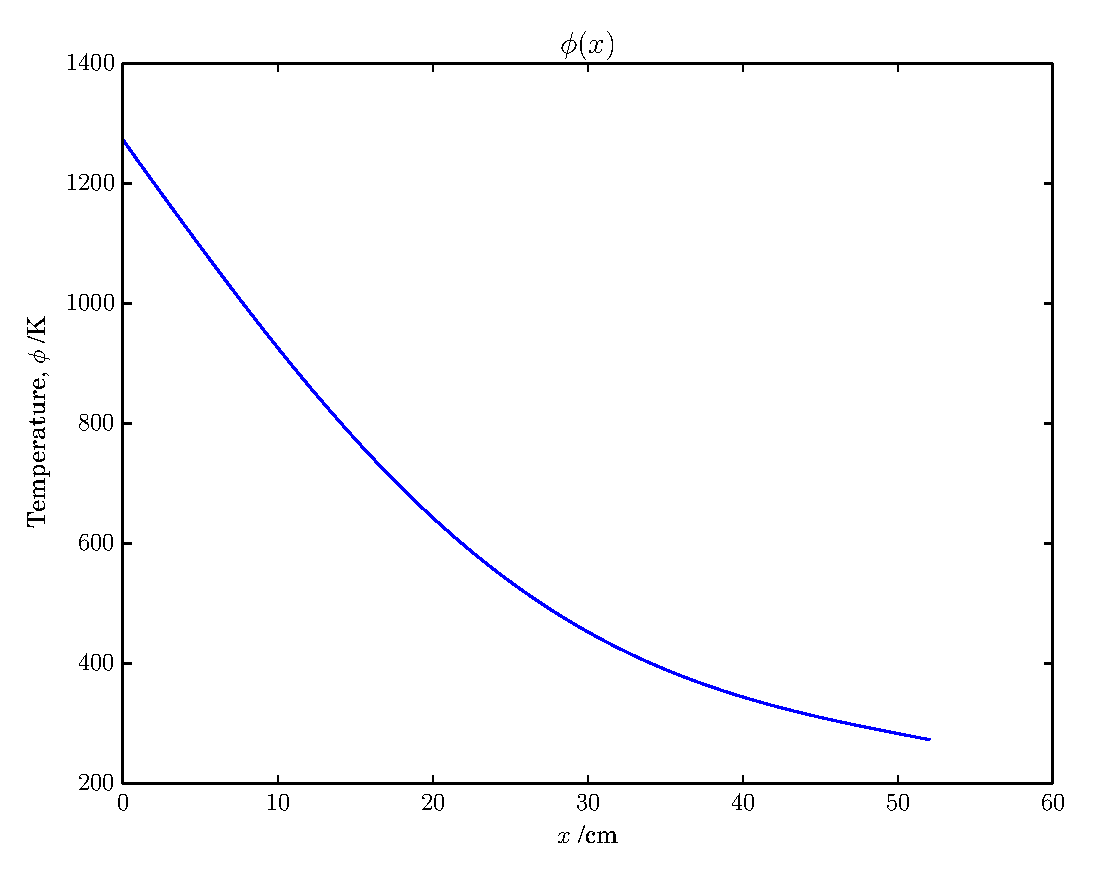
\includegraphics[width=0.5\linewidth]{graphs/diffusion/cold/t_1000_rod_normal}
        \label{subfig:cold_t_1000_normal}
    }
    \subfloat[$t=$\SI{10000}{\second}]{
        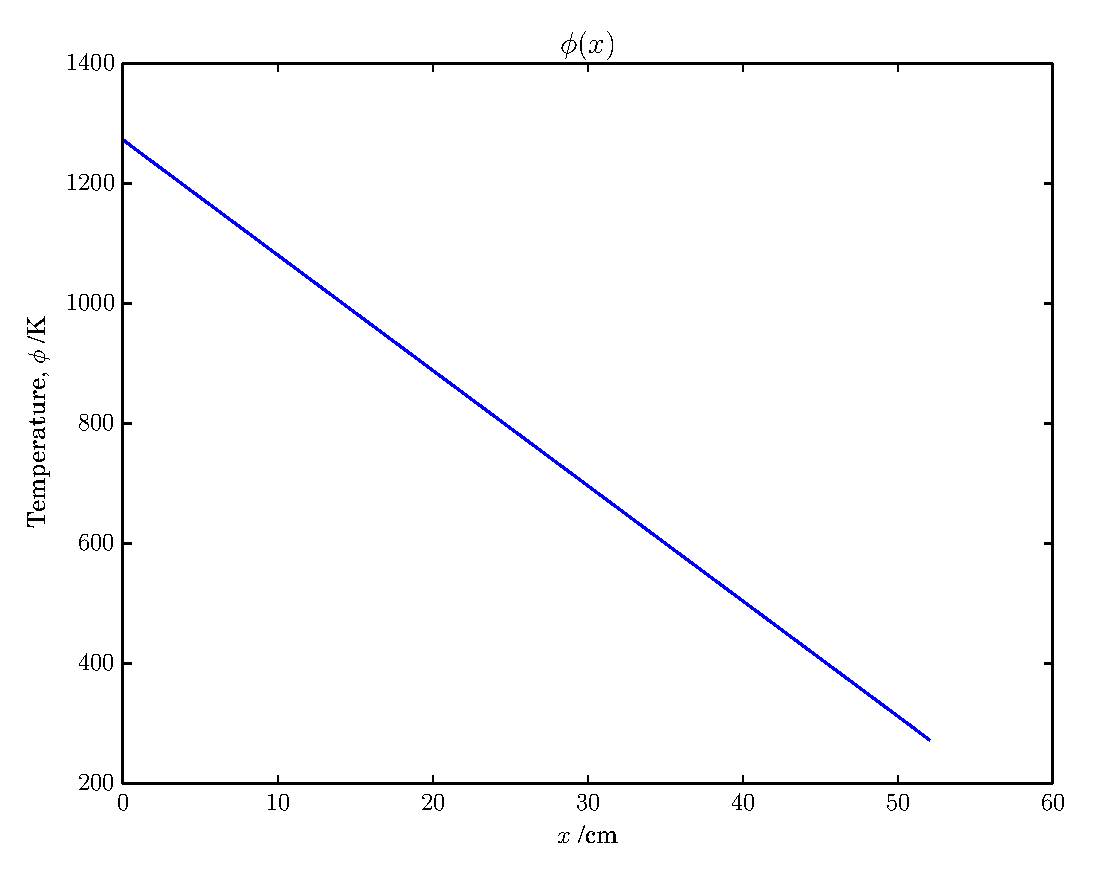
\includegraphics[width=0.5\linewidth]{graphs/diffusion/cold/t_10000_rod_normal}
        \label{subfig:cold_t_10000}
    }
    \caption{Temperature distribution along rod with one end in furnace and other in ice at \SI{1000}{\second} and \SI{10000}{\second}.}
    \label{fig:cold_diffusion}
\end{figure}

\subsection{Imposing Boundary Conditions}
\label{subsec:imposing_boundary_conditions}

Two boundary conditions need be imposed for this solution. The first type, Dirichlet boundary conditions, are the constant temperature regions, namely the $\phi(0,t)=\SI{1273.15}{\kelvin}$ for all $t$ in Section \ref{subsec:hot} and in addition $\phi(x_{\text{end}},t)=\SI{273.15}{\kelvin}$ for all $t$ in Section \ref{subsec:cold}. These are simple to impose as they can simply be set after every iteration. However, the second type of boundary conditions, the Neumann boundary conditions, are harder to implement. Here the Neumann boundary conditions are the no heat loss condition, which requires that $\frac{\partial \phi}{\partial x} = 0$ at the end of the rod. This is implemented by the altering of the top-left most and bottom-right most terms in the matrix of prefactors. Equation \ref{eqn:implicit}, giving the implicit BTCS method for iteration, gives a matrix of prefactors where every diagonal term is equal to $1+\frac{2\alpha\delta t}{h^2}$. The factor of 2 arises because the nearest two neighbours are taken into account. However, when talking about the first and last nodes, because no heat loss through the sides is desired, only the one neighbour should be taken into account and thus this term should be $1+\frac{\alpha\delta t}{h^2}$ instead. This takes the Neumann boundary conditions into account and removes the element of heat loss through the sides of the iron rod.

\subsection{Performance}
\label{subsec:performance}

In order to maximise the efficiency of the calculations, the matrix of prefactors is constructed and inverted in the main loop of the program. This means that this relatively processor intensive activity need take place only once at the beginning of the program, instead of whenever the system of linear equations is being solved to advance time by the time step at every iteration. This means instead of using \texttt{NumPy}'s \texttt{numpy.solve(a,b)} in every iteration, \texttt{numpy.linalg.inv()} is invoked once and in every iteration the rod at time $t$ is dotted with the inverse of the prefactor matrix to solve the set of linear equations and evolving time.

\section{Conclusion}
\label{sec:conclusion}

In conclusion, finite difference betweens are used to solve both Laplace's equation and the heat diffusion equation. The Laplace solution is then applied to the physical situation of a parallel plate capacitor, where it is shown that the infinite plate solution holds when the ratio of the width of the capacitor plates to the plate separation is sufficiently large. Finally the solution to the heat diffusion equation is applied to the case of an iron rod with one end in a hot furnace and the other end in and out of freezing water. It is demonstrated that only when one end is placed in ice that an equilibrium is found at finite time.